\chapter{Linear support vector machines}
\label{ch:linear-svm}

\begin{learningobjectives}
After this chapter, you should be able to:
\begin{itemize}
  \item express a linear support vector machine as a single-neuron model while
  distinguishing its loss and output semantics from regression models;
  \item derive the distance from a point to a hyperplane and the width of the
  canonical margin;
  \item pass from hard-margin constraints to slack variables and hinge loss;
  \item calculate a valid subgradient of the regularized hinge objective;
  \item explain the roles of scaling, regularization, and support vectors; and
  \item evaluate margin scores without misrepresenting them as probabilities.
\end{itemize}
\end{learningobjectives}

\begin{chapterconnection}
Chapter~\ref{ch:classification} used a sigmoid single neuron to model a
conditional probability. A linear support vector machine begins with the same
affine preactivation $z(x)=w^Tx+b$, but asks a different question: can we find
a separating hyperplane with a wide, violation-tolerant margin? This third
single-neuron configuration will make the shared structure---and the important
differences---visible before Chapter~\ref{ch:learning-api} turns that structure
into a software design.
\end{chapterconnection}

The chapter follows one continuous argument. An affine score produces a
hyperplane. Orthogonal projection turns that score into distance. Normalizing
the otherwise arbitrary parameter scale produces a geometric margin.
Maximizing that margin produces the hard-margin optimization problem. Finally,
slack variables repair infeasible constraints and become hinge loss. Each new
formula will answer a geometric problem created by the preceding one.

\section{One affine neuron, a different objective}

For an observation $x\in\mathbb R^p$, define
\[
  z(x)=w^Tx+b.
\]
The sign of $z(x)$ selects a class, and the zero level set
$H=\{x:w^Tx+b=0\}$ is the decision hyperplane. We use signed targets
$y_i\in\{-1,+1\}$. The product $y_i z_i$ is positive precisely when the
score has the correct sign. This product will become the organizing quantity
for the chapter.

The neuron is therefore familiar, but its learning rule is not yet specified.
Linear regression couples the affine score to squared loss, and logistic
regression couples a sigmoid postactivation to log loss. A linear SVM will
couple the affine score to signed labels, geometric margin, regularization, and
hinge loss. The point is not to attach a new name to the same model; it is to
reuse a computation while changing the mathematical problem.

\begin{misconceptionbox}
\textbf{Misconception:} sharing the affine formula makes these models
mathematically equivalent. \textbf{Correction:} the activation, target space,
loss, regularization, optimizer, and output interpretation are part of the
model. Reusing one computation does not erase those differences.
\end{misconceptionbox}

\section{Geometry of a separating hyperplane}

First establish the geometry rather than memorizing a distance formula. If
$u,v\in H$, then
\[
  w^Tu+b=0,\qquad w^Tv+b=0.
\]
Subtracting gives $w^T(u-v)=0$. Every displacement $u-v$ along $H$ is
therefore perpendicular to $w$: the weight vector is the normal direction.
Moving parallel to $H$ leaves the score unchanged, while moving in the $w$
direction changes it most rapidly.

\begin{proposition}[distance to a hyperplane]
For $w\ne 0$, the Euclidean distance from $x$ to $H$ is
\[
  \operatorname{dist}(x,H)=\frac{|w^Tx+b|}{\lVert w\rVert_2}.
\]
\end{proposition}

\begin{proof}
Let $x_H$ be the orthogonal projection of $x$ onto $H$. The shortest
displacement is perpendicular to $H$, so write $x-x_H=tw$. Since
$w^Tx_H+b=0$,
\[
  w^Tx+b=w^T(x-x_H)=t\lVert w\rVert_2^2.
\]
Therefore $|t|=|w^Tx+b|/\lVert w\rVert_2^2$, and
$\lVert x-x_H\rVert_2=|t|\lVert w\rVert_2$ gives the result.
\end{proof}

For a concrete calculation, take $w=(2,-1)^T$, $b=-1$, and
$q=(2,1.5)^T$. Then $z(q)=1.5$, $\lVert w\rVert_2=\sqrt5$, and
\[
  q_H=q-\frac{z(q)}{\lVert w\rVert_2^2}w=(1.4,1.8)^T.
\]
Indeed, $2(1.4)-1.8-1=0$, so $q_H\in H$, and the distance is
$1.5/\sqrt5\approx0.671$. Figure~\ref{fig:svm-hyperplane-geometry}A shows
the point, its projection, the normal, and the displacement used in the proof.

\subsection{Functional and geometric margin}

For signed label $y_i$, define the \term{functional margin}
$m_i=y_i(w^Tx_i+b)$. Its sign records correctness, but its magnitude is not a
distance. Replacing $(w,b)$ by $(cw,cb)$ for any $c>0$ leaves the hyperplane
and every decision unchanged while multiplying $m_i$ by $c$. The geometric
signed margin removes that arbitrary scale:
\[
  \gamma_i=\frac{y_i(w^Tx_i+b)}{\lVert w\rVert_2}.
\]
Under the same rescaling, both numerator and denominator acquire a factor
$c$, so $\gamma_i$ is unchanged. This is the distinction visualized in
Figure~\ref{fig:svm-hyperplane-geometry}B.

\subsection{Canonical scaling and the hard margin}

Suppose the data are linearly separable. Among all positive rescalings of a
fixed separating boundary, choose the canonical one satisfying
\[
  \min_i y_i(w^Tx_i+b)=1.
\]
At least one observation from each side then touches a supporting level
$w^Tx+b=+1$ or $w^Tx+b=-1$. These observations are the first support vectors.
Canonical scaling does not move the decision boundary; it merely chooses one
representative from an otherwise redundant family of parameter vectors.

\begin{proposition}[canonical margin width]
The distance between the planes $w^Tx+b=1$ and $w^Tx+b=-1$ is
$2/\lVert w\rVert_2$.
\end{proposition}

\begin{proof}
Each plane lies $1/\lVert w\rVert_2$ from the central plane by the preceding
proposition. They lie on opposite sides, so the distances add.
\end{proof}

The factor $2$ is fixed, so maximizing width is equivalent to minimizing
$\lVert w\rVert_2$. Squaring the norm and multiplying by $1/2$ preserve the
minimizer and give a convenient convex objective. Canonical scaling supplies
the constraints, producing
\[
  \min_{w,b}\frac12\lVert w\rVert_2^2
  \quad\text{subject to}\quad
  y_i(w^Tx_i+b)\ge 1,\qquad i=1,\ldots,n.
\]
This is the hard-margin SVM. The objective widens the band; the constraints
keep every training point on the correct side of its supporting level.
Figure~\ref{fig:svm-hyperplane-geometry}C shows both roles. The zero vector
cannot minimize the problem because it violates every constraint.

\begin{figure}[htbp]
  \centering
  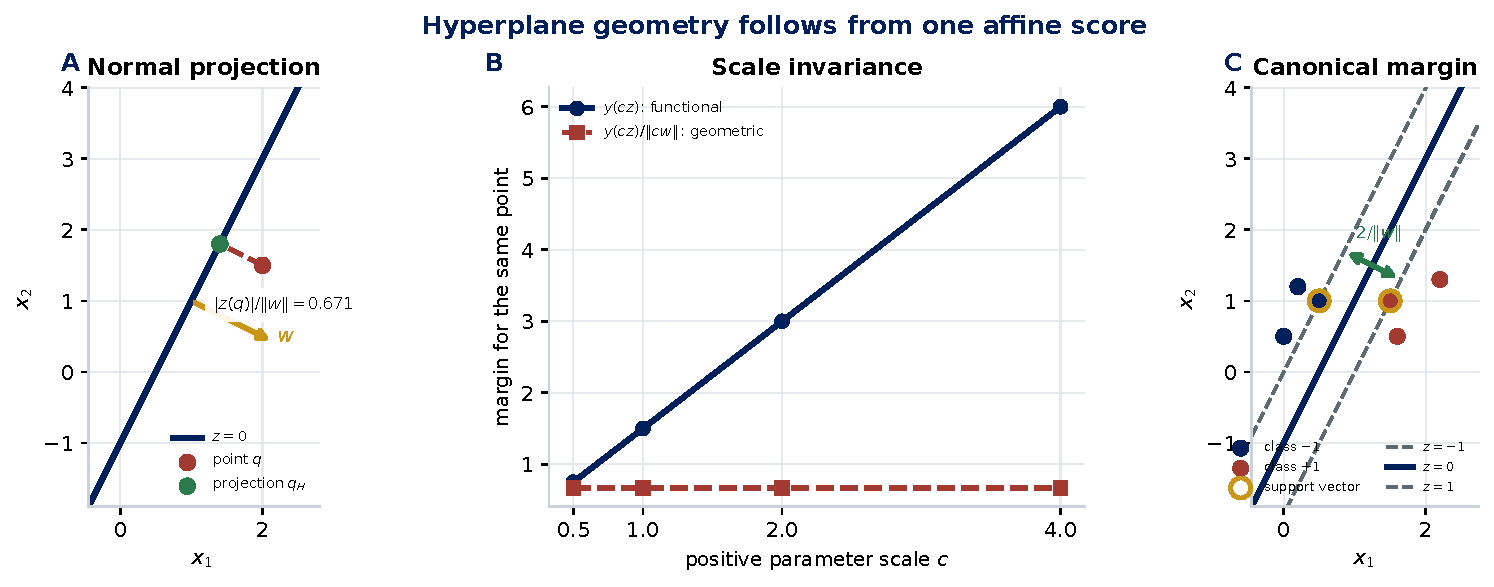
\includegraphics[width=\textwidth]{figures/generated/svm-hyperplane-geometry.pdf}
  \caption{The derivation of maximum-margin geometry for
  $z(x)=2x_1-x_2-1$. \textbf{A:} Orthogonal projection onto $z=0$ follows the
  normal $w$ and gives distance $|z(q)|/\lVert w\rVert_2$. \textbf{B:}
  rescaling $(w,b)$ changes functional margin but not normalized geometric
  margin. \textbf{C:} canonical scaling places the closest observations on
  $z=\pm1$; the perpendicular distance between these supporting levels is
  $2/\lVert w\rVert_2$. The figure is generated by the same NumPy and
  Matplotlib construction used in Lecture 11 notebook 01.}
  \label{fig:svm-hyperplane-geometry}
\end{figure}

\conceptcheck{Why can we not maximize a meaningful geometric margin merely by
multiplying both $w$ and $b$ by a large constant? Which normalization removes
that ambiguity?}

\section{Soft margins lead to hinge loss}

The hard-margin problem has a serious failure mode: one overlapping or
mislabeled observation can make all constraints jointly infeasible. We retain
the desired unit margin but permit observation $i$ to fall short by a
nonnegative slack $\xi_i$:
\[
  y_i(w^Tx_i+b)\ge 1-\xi_i.
\]
Rearranging gives $\xi_i\ge1-y_i z_i$, while nonnegativity also requires
$\xi_i\ge0$. Therefore, at fixed $(w,b)$, the smallest feasible slack is
\[
  \xi_i=\max\{0,1-y_i(w^Tx_i+b)\}.
\]
This is the hinge loss $\ell_{\mathrm{hinge}}(y_i,z_i)$. Its three regions
have direct geometric meanings:
\begin{itemize}
  \item $y_i z_i>1$: correctly classified beyond the margin, so $\xi_i=0$;
  \item $0<y_i z_i<1$: correctly classified but inside the margin, so
  $0<\xi_i<1$; and
  \item $y_i z_i\le0$: on the boundary or misclassified, so $\xi_i\ge1$.
\end{itemize}

\begin{proposition}[slack--hinge equivalence]
For fixed $(w,b)$, minimizing $\sum_i\xi_i$ subject to
$\xi_i\ge0$ and $\xi_i\ge1-y_i z_i$ produces
$\xi_i=\max(0,1-y_i z_i)$ for every $i$.
\end{proposition}

\begin{proof}
Each $\xi_i$ must be at least both $0$ and $1-y_i z_i$. Their maximum is the
smallest feasible value. Any larger value increases the objective without
improving feasibility.
\end{proof}

We use the averaged objective
\[
 J(w,b)=\frac{\lambda}{2}\lVert w\rVert_2^2
 +\frac1n\sum_{i=1}^n\max\{0,1-y_i(w^Tx_i+b)\}.
\]
Larger $\lambda$ favors a smaller weight norm and therefore a wider margin,
while permitting more violations. Many libraries instead use
$\tfrac12\lVert w\rVert^2+C\sum_i\xi_i$; larger $C$ then penalizes violations
more strongly. The convention, and whether the loss is summed or averaged,
must be documented.

\section{Subgradients and first-order training}

The geometry has now produced an objective. Training requires the direction in
which that objective changes. This calculation also explains computationally
why only observations near the boundary determine the fitted solution.

Hinge loss is convex but not differentiable at signed margin $y_i z_i=1$.
Away from that kink,
\[
 \frac{\partial \ell_i}{\partial z_i}=
 \begin{cases}
   -y_i,&y_i z_i<1,\\
   0,&y_i z_i>1.
 \end{cases}
\]
If $A=\{i:y_i z_i<1\}$ is the active set, a valid batch subgradient is
\[
 g_w=\lambda w-\frac1n\sum_{i\in A}y_i x_i,
 \qquad
 g_b=-\frac1n\sum_{i\in A}y_i.
\]
At the kink, any value between the one-sided slopes is valid; an
implementation must choose and test a convention. A subgradient step is
$(w,b)\leftarrow(w,b)-\eta(g_w,g_b)$.

\begin{warningbox}
A decreasing training objective is an implementation check, not proof of
generalization. Selection and reporting still require held-out data, comparison
with baselines, subgroup analysis, and metrics chosen for the deployment cost.
\end{warningbox}

\section{Support vectors, scaling, and scores}

The active set $A$ in the preceding formula is the algebraic version of the
orange-ringed observations in Figure~\ref{fig:linear-svm-margin}. Only
observations on or inside the unit margin have nonzero hinge
subgradients. At a solution, these support vectors determine the boundary;
points far beyond the margin do not directly contribute to the hinge term.
This sparsity is geometric, not a license to ignore provenance or data quality.

Feature scaling is essential. A Euclidean norm on $w$ and a geometric margin
depend on feature units. If one feature is measured in micrometers and another
in thousands of dollars, the unscaled penalty silently imposes an arbitrary
geometry. Fit a scaler on training data only, reuse it unchanged on validation
and test data, and retain feature names and units.

\subsection{Scores are not probabilities}

The raw score $z=w^Tx+b$ ranks distance in the direction normal to the
boundary, but it is not a probability. If calibrated probabilities are needed,
calibration is a separate model-selection step fitted without contaminating the
final test set.

\begin{workedexample}{margin status for three observations}
Suppose a fitted standardized model produces signed margins
$y_i z_i\in\{-0.4,0.6,1.7\}$. Their hinge losses are respectively
$1.4$, $0.4$, and $0$. The first is misclassified, the second is correctly
classified but inside the margin, and the third is correctly classified beyond
the margin. The first two influence the current hinge subgradient; the third
does not. Logistic loss, by contrast, remains positive at every finite margin.
\end{workedexample}

\begin{figure}[htbp]
  \centering
  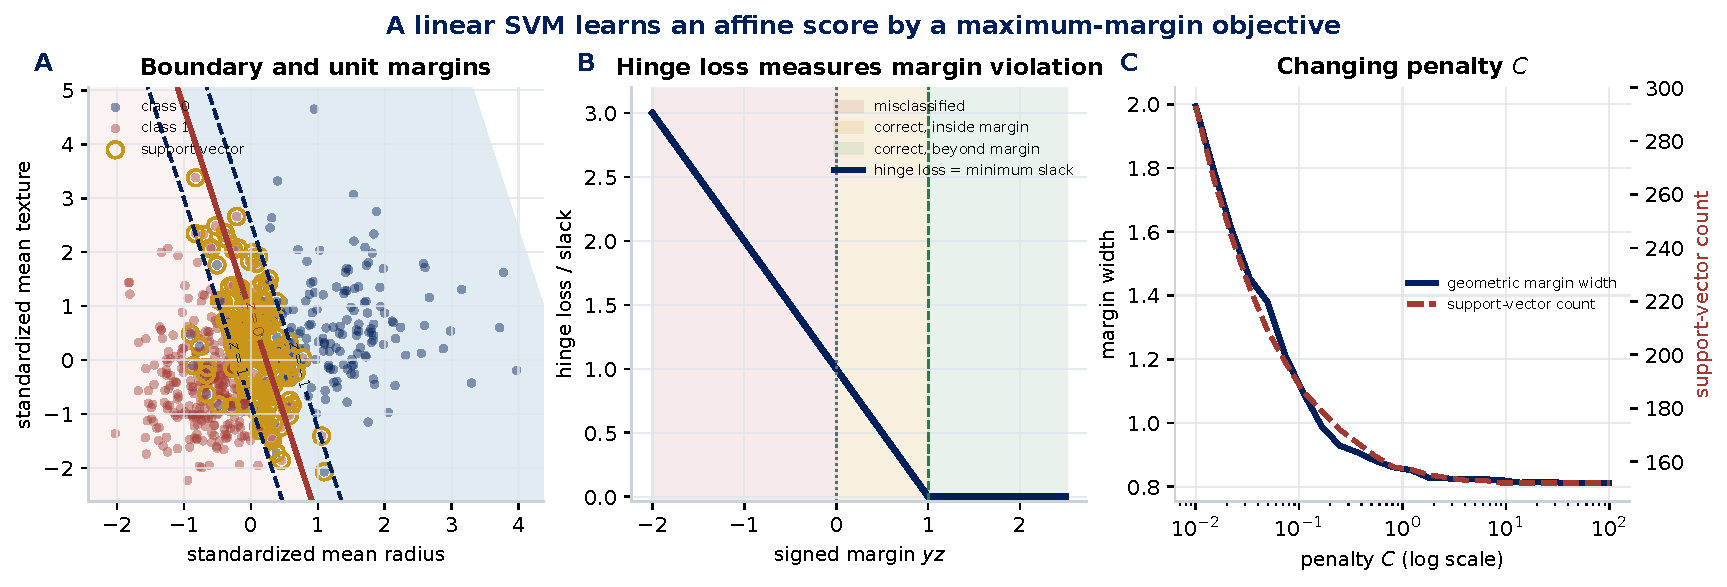
\includegraphics[width=\textwidth]{figures/generated/linear-svm-margin.pdf}
  \caption{A linear SVM fitted to versioned diagnostic measurements. Left:
  decision boundary, unit margins, and support vectors. Center: the three
  geometric regions of signed margin and the hinge loss each produces. Right:
  regularization changes margin width and the number of active observations.}
  \label{fig:linear-svm-margin}
\end{figure}

\section{Professional evidence workflow}

A defensible linear-SVM experiment records the target definition, data query,
split identifiers, preprocessing fitted on the training partition, feature
units, label encoding, objective convention, hyperparameters, convergence
trace, and held-out metrics. Report the confusion matrix at the operational
threshold and discuss which errors matter. Compare with logistic regression:
similar discrimination does not make a margin score a calibrated probability.

\begin{professionalbox}
Treat the model and preprocessing as one fitted pipeline. Persist them
together, validate input schema at inference, monitor score and feature drift,
and log model and data versions. Unit tests should cover label validation,
unfitted-state errors, output shapes, deterministic training, and a small
separable problem with a known qualitative solution.
\end{professionalbox}

\section{Exercises}

\begin{enumerate}
  \item Compute the geometric distance of $x=(2,1)$ from
  $2x_1-x_2-3=0$. Then rescale all coefficients by $5$ and verify that the
  distance is unchanged.
  \item For signed margins $-2,-0.2,0,0.8,1,2$, calculate hinge and logistic
  loss. Explain which observations influence the hinge subgradient.
  \item Starting from the soft-margin constrained problem, eliminate the slack
  variables and recover the hinge objective.
  \item Derive $g_w$ and $g_b$ for one observation in each of the three regions:
  misclassified, correctly classified inside the margin, and beyond the margin.
  \item Fit a linear SVM and logistic regression to the same database query.
  Use one frozen split and one fitted scaler. Compare ranking, confusion
  matrices, calibration evidence, and failure cases.
  \item Add a test that would fail if an implementation regularized its bias.
  State why the desired behavior is part of the estimator contract.
\end{enumerate}

\begin{chapterreview}
A linear SVM is a single-neuron model with affine preactivation, signed labels,
and a regularized hinge objective. Hyperplane geometry explains the margin;
slack variables explain hinge loss; subgradients permit first-order training;
and support vectors identify active constraints. The shared affine computation
connects SVMs to linear and logistic regression, while their losses and output
semantics keep the estimators distinct.
\end{chapterreview}

\begin{notebooklink}
Lecture 11 notebook 01 derives these results, queries the course database,
visualizes margins and support vectors, trains the course implementation, and
evaluates held-out evidence. Lecture 12 notebook 00 then uses the three
single-neuron configurations to motivate reusable software design.
\end{notebooklink}
